\documentclass[a4paper, oneside]{book}
%Use package definitions
\usepackage[margin=1.4in]{geometry}
\usepackage[utf8]{inputenc}
%Serif font
\usepackage{cmbright}
\usepackage[T1]{fontenc}
\usepackage{textcomp}
\usepackage{amsmath, amssymb, bm}
\usepackage{pdfpages}
%Line through stuff
\usepackage{centernot}
\usepackage{transparent}
\usepackage{varwidth}
%Custom boxes
\usepackage[most]{tcolorbox}
\usepackage{xcolor}
\usepackage{url}
\usepackage{hyperref}
%Algorithm environments
\usepackage{algorithm}
\usepackage{algpseudocode}
%Header
\usepackage{titleps}

\newpagestyle{main}{
\setheadrule{.4pt}% Header rule
\sethead{MATH70027 Project 2 Solutions}{}{CID: 01859216}
% \setfootrule{.4pt}
\setfoot{}{\thepage}{}
}
\pagestyle{main}
%Space between paragraphs
\setlength{\parskip}{10pt}
%No indentation on the first word of a new paragraph
\setlength{\parindent}{0cm}
%Creating a new color box
\newtcolorbox{blackbox}[1][]{colframe=black,colback=white,sharp corners,center,#1}
%Creating the title

%Creating the title
\title{MATH70027 - Scientific Computation Project 2 Solutions\author{CID: 01859216}\date{\today}}


% -----------------------------------------------------------------------
\begin{document}
\maketitle


\section*{Part 1}
\subsection*{Q1.}
These functions return $d \in \mathbb{Z}$, which represents the maximum weight along the path with minimum maximum weight. So instead of finding the "shortest path" (path with smallest sum of edge weights) these algorithms find the path with the smallest maximum weight.
For example if we have the following graph:

\begin{figure}[htpb]
    \centering
    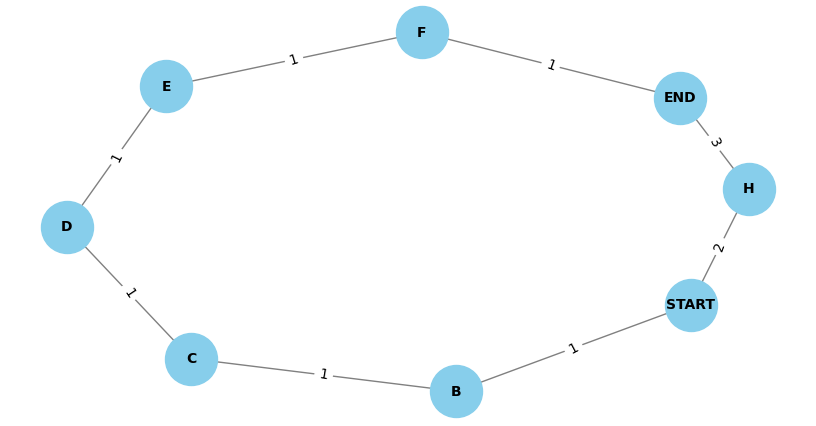
\includegraphics[width=0.8\textwidth]{./images/example_graph.png}
    \caption{Example graph.}
\end{figure}

And we set source to be START and target to be END, then traditional Dijkstra's for shortest
path would return 2 + 3 = 5 with path ["START", "H", "END"] but this modified version returns
max(1, 1, 1, 1, 1, 1) = 1 with path ["START", "B", "C", "D", "E", "F", "END"].
searchGPT also returns a list which represents nodes in the min-max path in order from source to target node.
This is a modified version of Dijkstras', which takes the maximum instead of the sum of
weights along the min-max path. This is done with a greedy approach, (using a priority queue) with edges with smaller distances visited first. We start at the source node and set this to the current node and then iteratively consider the neighbouring nodes, updating our "distances" as the max distance along the current path from the source to current node as we go.

Once the current node is the target node, we are guaranteed to have found the min-max path, since if we have reached the target node but there was some alternate path with
smaller maximum weight then by definition of the priority queue this node with smaller
max weight should have been popped from the priority queue first and so this is not possible.

SearchGPT also keeps track of the parent of each node in the current best min-max path
and so once we reach the target node we step backward through the dictionary in order to
reconstruct the min-max path.


\subsection*{Q2.}

So in order to return the same list as searchGPT (a.k.a the ordered list of nodes that
appear in the min-max path), we need to keep track of the parents of each node that we
visit that appears in the optimal path. We do this using a dictionary `parents` that maps
the node to it's parent node. We do this update everytime we push to the priority queue.
Then once we have hit the target node we step backwards through the parents dict
and reconstruct the path, similar to the code from searchGPT.

Clearly they are both a modified version of Dijkstra's and so we can just extend the general
proof of correctness from the lecture notes (Assuming nodes are reachable).
This works because, like +, max also preservers total ordering (for positive edge weights).

One thing to note is that searchGPT will always
return float("inf") if no path exists from source to target, however for searchPKR if no path
exists then the behaviour is not correct and when we return dmin we will just be returning
the last value of dmin before our priority queue became empty. 

 
In terms of computational cost, both implementation use a heap queue priority queue.
Both pushing to and popping from a heapq in python have time complexity $O(\log_{2}N)$ where 
$N$ is the length of the queue.

Suppose our graph has $N$ nodes and $L$ edges, then we have worst case computational time complexity: $O(N\log_{2}N + L \log_{2}N)$ since in the worst case we will have to visit all nodes, thus
popping $O(N)$ times (visiting a node corresponds to popping that node from the priority queue). Then pushing $O(L)$ times, due to iterating over neighbouring nodes for each current node.

We also have to consider the computational cost of re-constructing the path.
In searchGPT this is done rather inefficiently, since we loop over all key-value pairs
in the parents dictionary and then push to the front of our path list.
In the worst case we could have $O(N)$ nodes in our path and then pushing
to the front of the path list will have time complexity $O(N)$, which means
in total we have $O(N^{2})$ time complexity for re-constructing the path in searchGPT.
So overall we have $O((N + L)\log_{2}N + N^{2})$ worst case time complexity for
searchGPT, and $O((N+L)\log_{2}N)$ worst case time complexity for searchPKR
since we aren't doing any path reconstruction.
Then for searchPKR2, our implementation, we implement a more efficient path
reconstruction algorithm. We still store the parents as is done in searchGPT
but then when we step through this dictionary, we first pre-allocate an array
and then when we step back through the parents we are just assigning values
and updating an index, instead of pushing to the front of a list. This brings
the computational time complexity down to $O(N)$ and so our searchPKR2 implementation
has $O((N+L)\log_{2}N + N) = O((N+L)\log_{2}N)$ worst case time complexity.

When it comes to memory complexity clearly the heap queue will have space complexity
worst case $O(N)$, but we also have to store the graph itself in memory, which will take
$O(N+L)$ so the overall memory complexity is $O(N+L)$.

In terms of differences, they both use different computation saving measures.
For each iteration, searchGPT checks if the current distance is greater than the stored
distance for the current node and if it is, this node is skipped. This will obviously 
reduce the number of unnecessary computations. Note that searchPKR
does not do this, but rather keeps track of previously visited finalized nodes using the
dictionary Fdict.

Note that these measures do not affect the worst-case computational complexity, but
will improve the wall times.

\section*{Part 2}
\subsection*{Q1.}
Firstly we can speed up the RHS function, since in part2q1 a for loop is used and for loops
are slow in python. To get around this we vectorize the operations. Numpy already has built
in vectorized element-wise multiplication, powers, addition and subtraction so we just have
to deal with the dependence on $y_{i-1}$ and $y_{i+1}$ for element $i$. We can also vectorize this using
the scipy shift function, which shifts the elements down/up and replaces the missing values
with whatever we pass to the cval argument. 
This means we get rid of the loop and then just define:
\begin{blackbox}
\begin{verbatim}
	y_prev = shift(y, 1, cval=0)
	y_next = shift(y, -1, cval=0)
	dydt = alpha * y - y**3 + beta * (y_next + y_prev)
\end{verbatim}
    
\end{blackbox}
(Then dealing with the 0 and n-1 index edge cases just as before).

Then the biggest speedup comes from switching out the iterative for loop method
with scipys' solve\_ivp method. We can just pass it our RHS function, the start and end
times, our initial conditions, the time values we want to evaluate at and our error tolerances.

Note that scipy keeps the error bounded by $\text{atol} + \text{rtol} * \text{abs}(\mathbf{y})$. According to the Scipy documentation, if we want to specify that the absolute error is less than $10^{-6}$ then we need to set $\text{atol} = 10^{-6}$ and then choose
$\text{rtol}$ such that $\text{rtol} * \text{abs}(y_{i}) \leq \text{atol} ~ ~ \forall i$.
We can do this by noticing that the $y$ values are all bounded by $1$, so it is sufficient to also set $\text{rtol} = 10^{-6}$.

\subsection*{Q2.}

We start by using our part2q1new function to calculate the solutions to the initial value problem. We then plot them where each line represents $y_{i}(t)$ for some $i \in [0:n-1]$.
\begin{figure}[htpb]
    \centering
    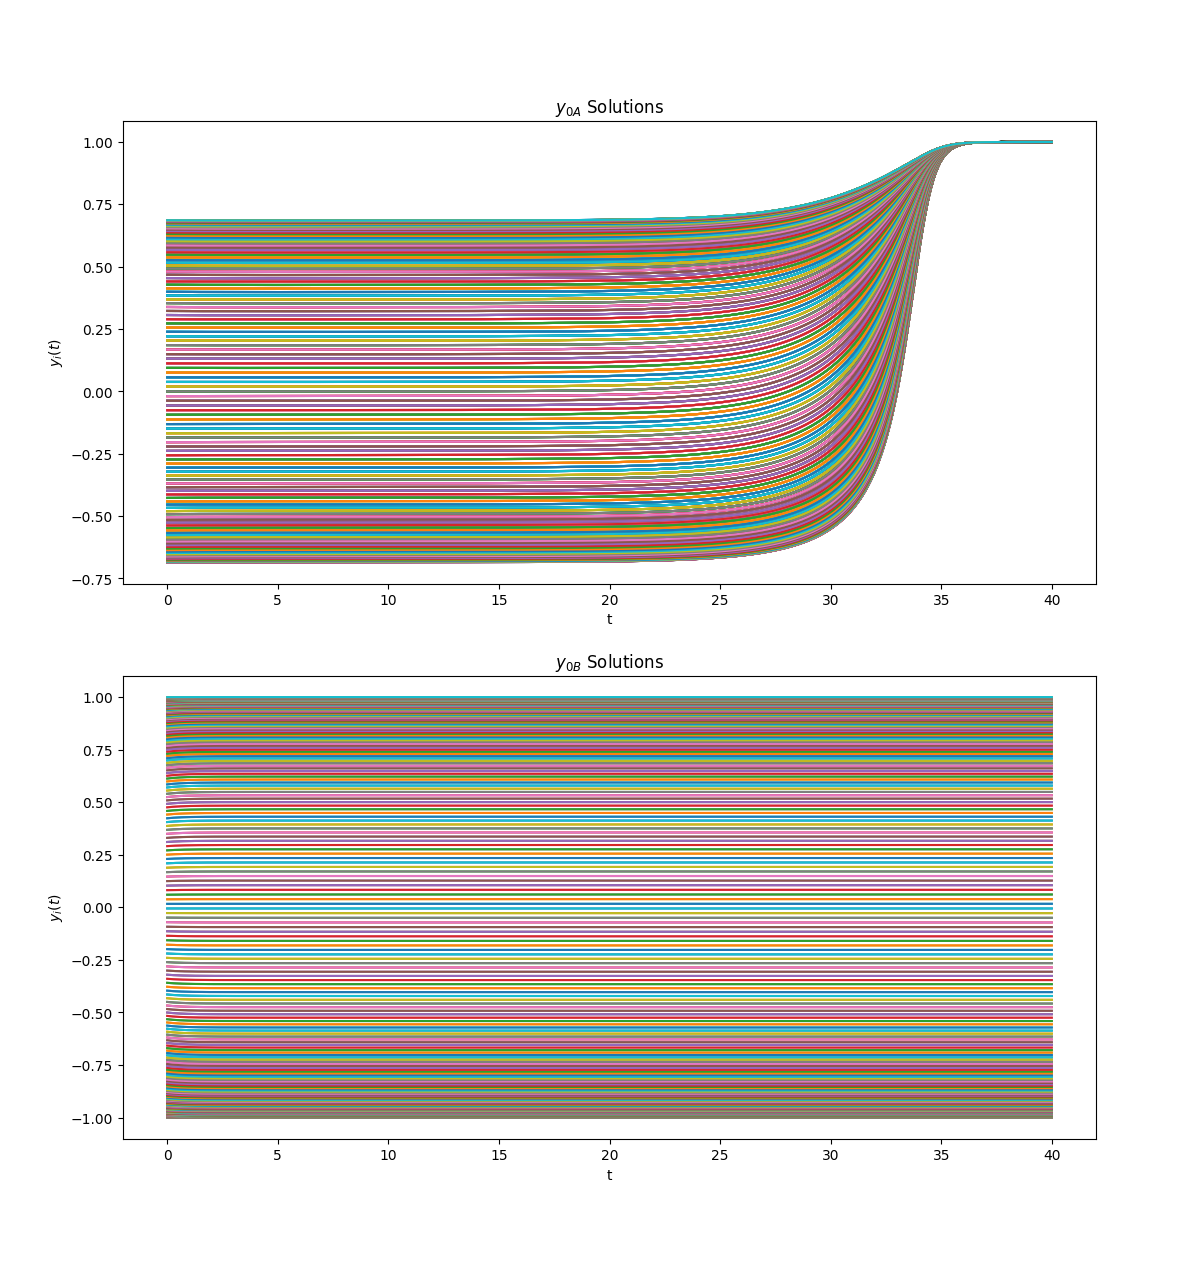
\includegraphics[width=1.0\textwidth]{./images/solutions.png}
    \caption{Solutions to the initial value problem using different initial conditions.}
\end{figure}

\clearpage

Qualitatively we we see that for $y_{0A}$ the $y(t)$ tends towards $y_{i} = 1 ~ ~ \forall i$, suggesting that this
is an attracting stable point. Then for $y_{0B}$ we notice that the $y(t)$ don't go to the $\bm{1}$ equilibrium
point, but rather almost instantly converge to a different equilibrium point, which we will
denote $\mathbf{y}^*$. 

Now examining why this might be, we turn to our system of equations:
Note that we are using $\beta := 10,000 / \pi^{2}$ and $\alpha :=  1 - 2\beta$. Plugging this into our system we get, 
\begin{align}
~ ~ \forall i \in [1:n-2], ~ ~
\frac{dy_{i}}{dt} &= (1 - 2\beta) y_{i} - y_{i}^{3} + \beta(y_{i-1} + y_{i+1}) \\
&= y_{i} - 2\beta y_{i} - y_{i}^{3} + \beta y_{i-1} + \beta y_{i+1} \\
	 & = y_{i} - y_{i}^{3} + \beta(y_{i-1} -2y_{i} + y_{i+1}) \\
\end{align}
And then looking at the edge cases we also have:
\begin{align}
\frac{dy_{0}}{dt} &= y_{0} - y_{0}^{3} + \beta(y_{n-1} - 2y_{0} + y_{1}) \\
\frac{dy_{n-1}}{dt} &= y_{n-1} - y_{n-1}^{3} + \beta(y_{0} -2 y_{n-1} + y_{n-2})
\end{align}
So immediately we notice that $y_{i} = 1 ~ ~ \forall i$ and $y_{i} = -1 ~ ~ \forall i$ and $y_{i} = 0 ~ ~ \forall i$ are all equilibrium
solutions. This clearly agrees with our qualitative analysis from our initial plots.

Another thing we notice is that if the differences between adjacent $y_{i}$'s are small then
the $\beta$ term becomes very small and the RHS is dominated by the $y_{i} - y_{i}^{3}$ term. In which case
as $y_{i+1} - y_{i} \to 0$ we get the system $\frac{dy_{i}}{dt} = y_{i} - y_{i}^{3}$, which has solutions that look like:

\begin{figure}[htpb]
    \centering
    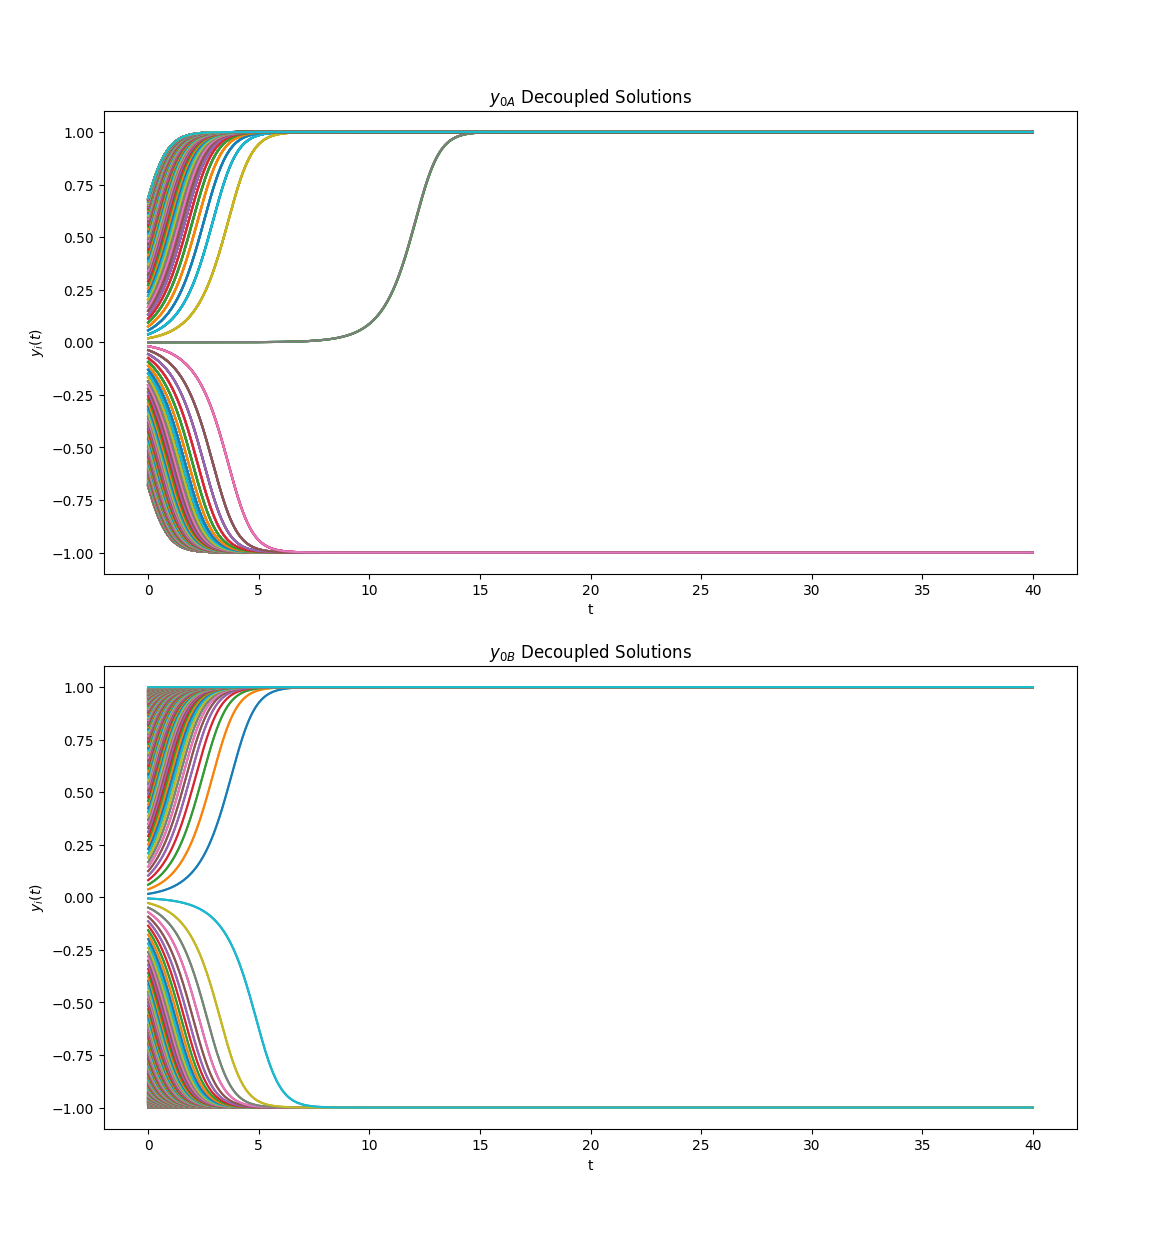
\includegraphics[width=1.0\textwidth]{./images/Pasted image 20231120143413.png}
    \caption{Solutions to the decoupled initial value problem with different initial conditions.}
\end{figure}
\clearpage

Which have the three stable points $y_{i} = 0 ~ ~ \forall i$, $y_{i} = -1 ~ ~ \forall i, y_{i} = -1 ~ ~ \forall i$. And clearly in this case,
both $y_{0A}$ and $y_{0B}$ tend to the same $y(t)$.

So the difference between the decoupled system and our system is that we also have
possible equilibrium points when $y_{i} - y_{i}^{3} = - \beta(y_{i-1} -2y_{i} + y_{i+1})$.

Clearly $\mathbf{y}^*$ is one such equilibrium point. In order to dig deeper into the difference between
the $y_{0A}$ initial condition solution and $y_{0B}$ initial condition solution we first look at the distribution of the initial conditions:
\begin{figure}[htpb]
    \centering
    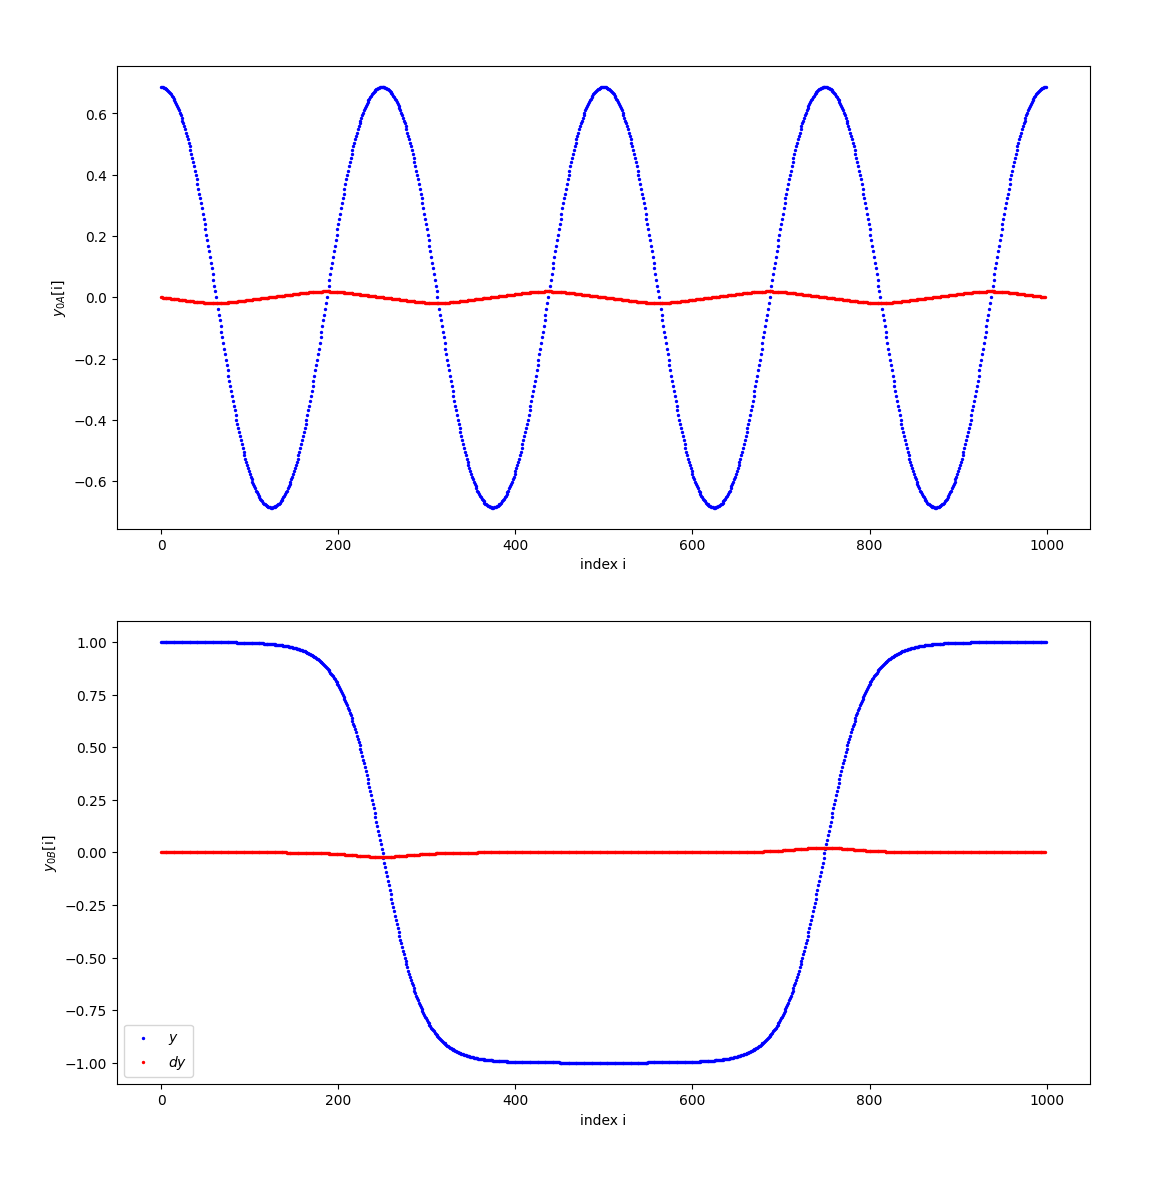
\includegraphics[width=1.0\textwidth]{./images/dist_of_init.png}
    \caption{}
\end{figure}
Note: the blue line represents $y_{0A/B}[i]$ against $i$ and the red line represents the first order
finite differences $y_{0A / B}[i + 1] - y_{0A / B}[i]$ against $i$. So we see that the initial conditions for $A$
oscillate much more between and also have max value around 0.6 and min value around -0.6. Whereas the initial conditions for $B$ oscillate less and have max values 1 and min values
-1. This is certainly interesting but doesn't immediately tell us why the solutions for
$y_{0A}$ and $y_{0B}$ converge to different equilibria.

In order to determine this we turn to perturbation theory and linearize our system. We
are mainly interested in the equilibrium point $\mathbf{y}^*$, since both $y_{0A}$ and $y_{0B}$ appear
to be close to this solution. So let:
$$
y_{i} = y_{i}^* + \epsilon \tilde{y_{i}} + O(\epsilon^{2})
$$
Then we have:
\begin{align}
\text{LHS} &= \frac{dy_{i}}{dt} = \epsilon \frac{d \tilde{y_{i}}}{dt} + O(\epsilon^{2}) \\
\text{RHS} &= y_{i} - y_{i}^{3} +\beta(y_{i-1} - 2y_{i} + y_{i+1}) \\
&= y_{i}^* + \epsilon \tilde{y_{i}} - (y_{i}^* + \epsilon   \tilde{y_{i}})^{3} + \beta(y_{i-1}^* + \epsilon  \tilde{y}_{i-1} - 2y_{i}^* - 2\epsilon \tilde{y}_{i} + y_{i+1}^* + \epsilon \tilde{y}_{i+1}) + O(\epsilon^{2}) \\
&= y_{i}^* - y_{i}^{*2} + \beta(y_{i-1}^* - 2y_{i}^* + y_{i+1}^*) + \epsilon (\tilde{y}_{i} - 3 y_{i}^{*2} \tilde{y}_{i} + \beta(\tilde{y}_{i-1} - 2 \tilde{y}_{i} + \tilde{y}_{i+1})) + O(\epsilon^{2})\\
&= \epsilon (\tilde{y}_{i} - 3 y_{i}^{*2} \tilde{y}_{i} + \beta(\tilde{y}_{i-1} - 2 \tilde{y}_{i} + \tilde{y}_{i+1})) + O(\epsilon^{2})\\
\end{align}
So dividing through by $\epsilon$ and letting $\epsilon \to 0$ we have:
$$
\frac{dy^*_{i}}{dt} = \tilde{y}_{i} - 3 y^{*2}_{i} \tilde{y}_{i} + \beta (\tilde{y}_{i-1} - 2 \tilde{y}_{i} + \tilde{y}_{i+1})
$$
and then for the edge cases we have:
\begin{align}
\frac{dy^*_{0}}{dt} &= \tilde{y}_{0} - 3 y^{*2}_{0} \tilde{y}_{0} + \beta (\tilde{y}_{n-1} - 2 \tilde{y}_{0} + \tilde{y}_{1}) \\
\frac{dy^*_{n-1}}{dt} &= \tilde{y}_{n-1} - 3 y^{*2}_{n-1} \tilde{y}_{n-1} + \beta (\tilde{y}_{0} - 2 \tilde{y}_{n-1} + \tilde{y}_{n-2})
\end{align}
So we can write this in matrix form. Define:
$$
M := \begin{pmatrix}
1-3y_{0}^{*2} - 2\beta & \beta & 0 & 0 & \dots & 0 & 0 & \beta \\
\beta & 1-3y_{1}^{*2} - 2\beta  & \beta & 0 & \dots & 0 & 0 & 0 \\
0 & \beta &   1-3y_{2}^{*2} - 2\beta  & \beta & \dots & 0 & 0 & 0 \\
\vdots  & \vdots  & \vdots & \vdots  & \vdots  & \vdots  & \vdots  & \vdots \\
0 & 0 & \dots  & 0 & \dots & \beta & 1-3y_{n-2}^{*2} - 2\beta  & \beta \\
\beta & 0 & \dots & 0 & \dots &  0 & \beta & 1-3y_{n-1}^{*2} - 2\beta
\end{pmatrix}
$$
Then we have:
$$
\frac{d \tilde{\mathbf{y}}}{dt} = M \tilde{\mathbf{y}}
$$
So if we find the eigenvalues $\lambda_{i}$ and eigenvectors $\mathbf{v}_{i}$ of $M$ then our solution will be:
$$
\tilde{\mathbf{y}}(t) = \sum_{i=0}^{n-1} c_{i} \mathbf{v}_{i} \exp(\lambda_{i} t)
$$
Where $c_{i}$ are constants to be determined using initial conditions. 
(Note: Since $M$ is real symmetric it must have $n$ linearly independent eigenvectors).

So $t = 0 \implies \tilde{\mathbf{y}}(0) = \sum_{i=0}^{n-1} c_{i} \mathbf{v}_{i} = V \mathbf{c}$ where we have defined $V$ to be the matrix with ith row
equal to the ith eigenvector of $M$. So to find $\mathbf{c}$ we have to solve $\tilde{y}(0) = V \mathbf{c}$ which we can
do using np.linalg.solve. So all that remains is to determine the initial conditions.

So if we assume that our initial conditions are close to the equilibrium point $\mathbf{y}^*$ then we have:
$$
\mathbf{y}(0) - \mathbf{y}^* = \epsilon \tilde{\mathbf{y}}(0)
$$
and then since the perturbation problem is linear, the magnitude of the initial condition
vector is inconsequential to our analysis and therefore we can use $\mathbf{y}(0) - \mathbf{y}^*$ as our initial
condition for the perturbed system.

Note: In order to get $\mathbf{y}^*$ we take the final time value of the array generated by solving 
the initial value problem with initial values given by $y_{0B}$.

Then in order to compare the behaviour with the different initial conditions, we solve
the above linearized system with $\mathbf{\tilde{y}}(0) := \mathbf{y}_{0A} - \mathbf{y}^*$ and then $\mathbf{\tilde{y}}(0) := \mathbf{y}_{0B} - \mathbf{y}^*$ and then plot
the resulting $\mathbf{\tilde{y}}(t)$ solutions:

\begin{figure}[htpb]
    \centering
    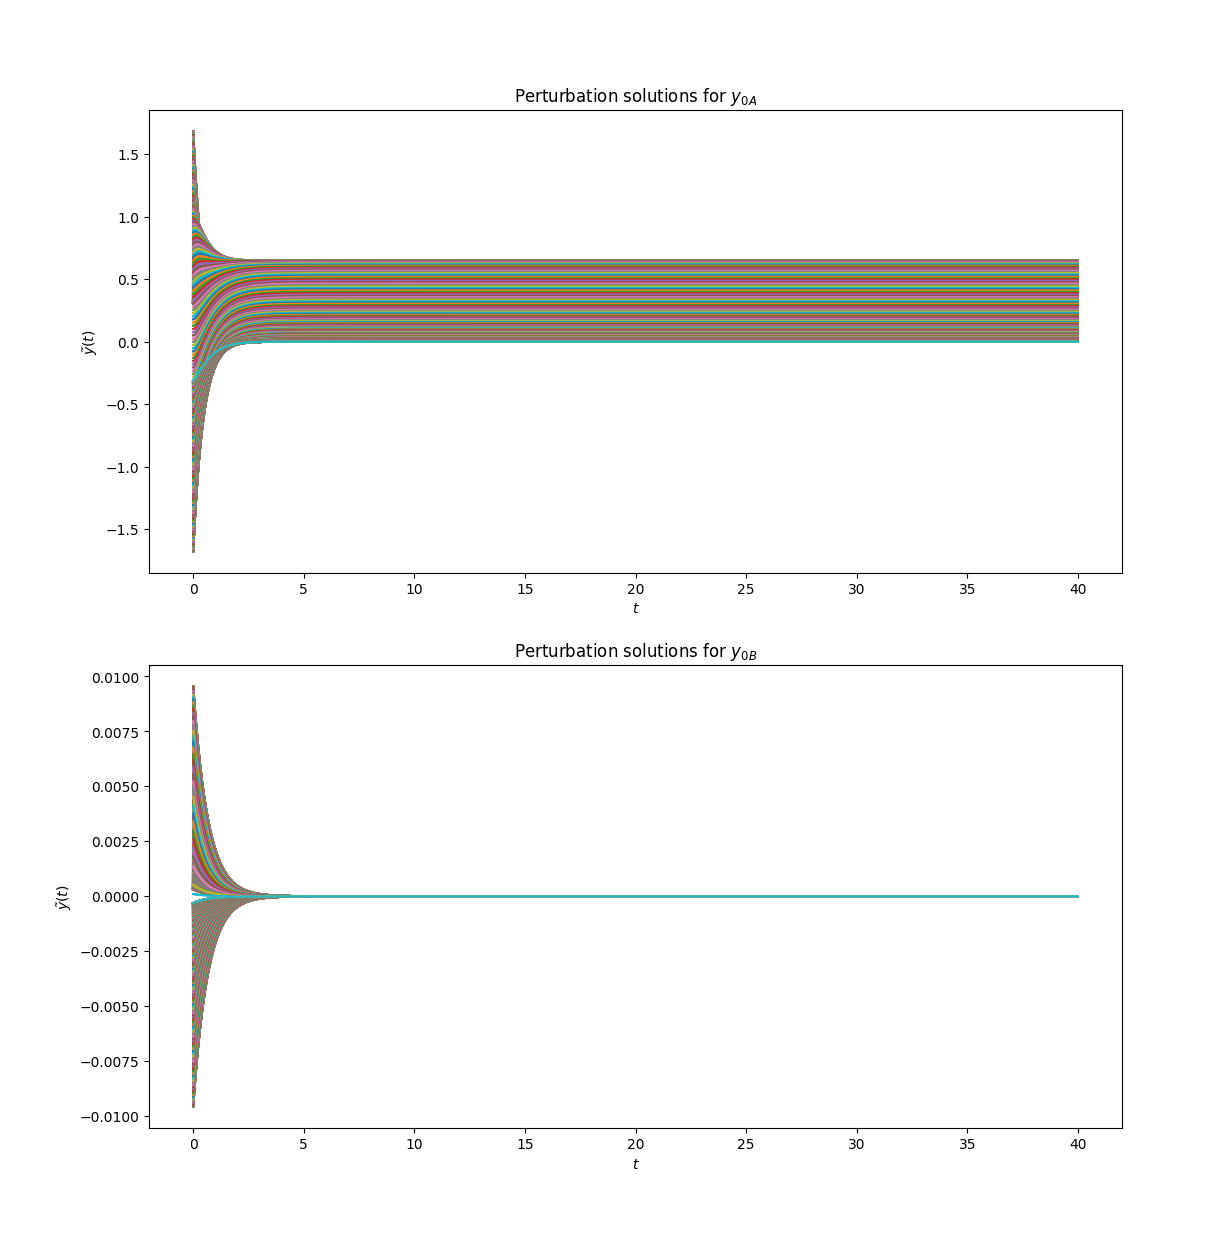
\includegraphics[width=1.0\textwidth]{./images/perturbation_solutions.png}
    \caption{Perturbation solutions for different initial conditions.}
\end{figure}
So we see that for initial conditions $y_{0A}$ the perturbations all converge to some
positive constant, whereas for initial conditions $y_{0B}$ all the perturbations converge to zero.
This result exactly supports our initial analysis, as we see that for $y_{0B}$ we converge almost
instantly to the equilibrium $\mathbf{y}^*$ and therefore stay there, without perturbation, whereas for $y_{0A}$ we converge to $\mathbb{1}$ and thus expect the perturbations to be positive constant.

\subsection*{Q3}
part2q3 is solving the following stochastic system:
\begin{align}
dy_{0} &= (y_{0} - y_{0}^{3} + \beta(y_{1} - 2 y_{0} + y_{2})) dt + \mu dW(t) \\
dy_{1} &= (y_{1} - y_{1}^{3} + \beta(y_{0} - 2 y_{1} + y_{2})) dt + \mu dW(t) \\
dy_{2} &= (y_{2} - y_{2}^{3} + \beta(y_{0} - 2 y_{2} + y_{1})) dt + \mu dW(t)
\end{align}
It is solving it by using the Euler-Maruyama (E-M) method:
$$
y_{i}^{(j+1)} = y_{i}^{(j)} + \Delta t * \text{RHS}(\mathbf{y}^{(j)})_{i} + \mu [W(t^{(j+1)}) - W(t^{(j)})]
$$
with $t^{(j)} = j \delta t$ and $W(t^{(j+1)}) - W(t^{(j)}) =  \sqrt{ \delta t } B_{i}$ where $B_{i} \sim \mathcal{N}(0, 1)$.

We plot the solutions for two different values of $\mu$:

\begin{figure}[htpb]
    \centering
    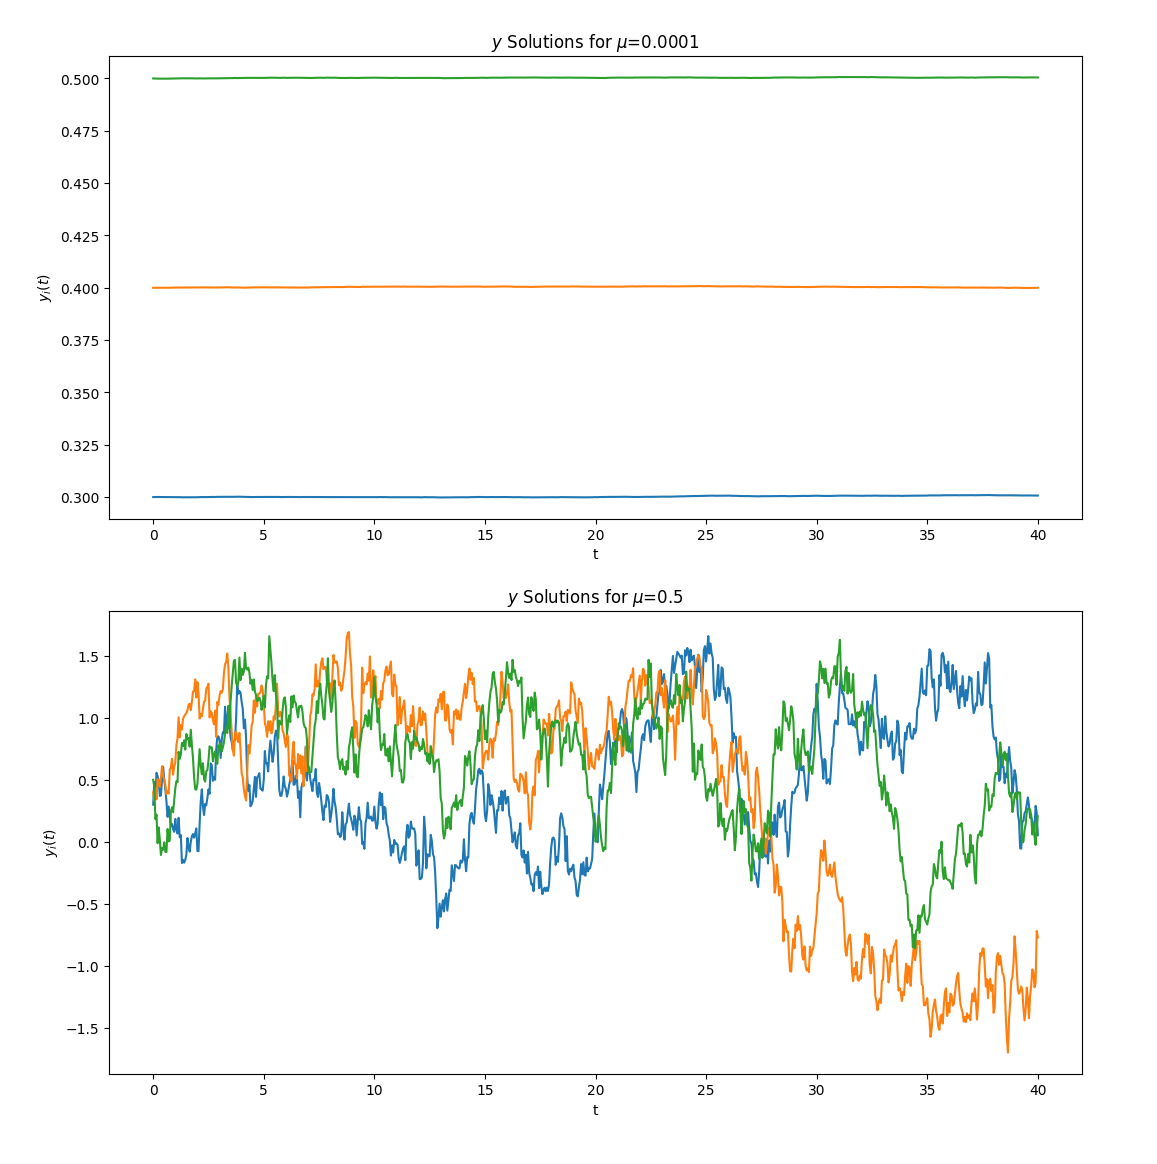
\includegraphics[width=0.8\textwidth]{./images/mu.png}
    \caption{Solutions for different values of $\mu$.}
\end{figure}

Clearly as $\mu \to 0$ we recover the deterministic system:

\begin{align}
\frac{dy_{0}}{dt} &= y_{0} - y_{0}^{3} + \beta(y_{1} - 2 y_{0} + y_{2})\\
\frac{dy_{1}}{dt} &= y_{1} - y_{1}^{3} + \beta(y_{0} - 2 y_{1} + y_{2})\\
\frac{dy_{2}}{dt} &= y_{2} - y_{2}^{3} + \beta(y_{0} - 2 y_{2} + y_{1}))
\end{align}
For which $(y_{0}, y_{1}, y_{2}) = \frac{1}{10}(3, 4, 5)$ is solution.

Then as we increase $\mu$ the brownian motion component starts to dominate
and the solution becomes more and more random.



% -----------------------------------------------------------------------
\end{document}
